\section{Methodology}
\label{appendix:method}
The formal diagnosis pipeline is shown in \cref{alg:diagnosis} and \cref{alg:multi_seed_quasi}. 

\paragraph{Greedy Multi-Seed Quasi-Clique Search}
As the identification of maximum cliques within the Interchangeability Graph is generally NP-hard, we implement a heuristic greedy search to approximate the interchange-consistent (perfectly interpreted) subspaces (\cref{alg:multi_seed_quasi}).
This algorithm serves as the implementation of the \textsc{FindMaximalQuasiClique} function within our diagnosis pipeline. 

To maximize the probability of discovering large dense regions, the algorithm employs a multi-seed strategy starting from the most promising candidates. %
We first compute the degrees of all nodes in $V \subseteq \mathcal{I}_{\mathrm{correct}}$ based on the current subgraph and sort them in descending order. %
The expansion is then attempted independently for each of the top 10 highest-degree nodes as seeds. %
For a given seed, the algorithm iteratively expands the set $C$ by selecting the candidate node $w$ that maximizes the resulting edge density $\rho$, provided that $\rho$ remains above the user-defined threshold $\gamma$. %

The density threshold $\gamma \in (0, 1]$ allows the framework to be robust to minor representational noise; while $\gamma=1.0$ identifies a perfect clique, a slightly lower value (e.g., $\gamma=0.9$) allows the pipeline to isolate regions of high causal faithfulness that might otherwise be fragmented by trivial neural variations. We choose $\gamma = 0.98$ for all experiments in the paper. 
The algorithm tracks the results of each seed and returns the largest quasi-clique $C_{\mathrm{best}}$, which is then extracted as a ``Target Bucket'' before the search space is updated for the next iteration. %

\begin{algorithm}[ht]
\caption{The Diagnosis Pipeline}
\label{alg:diagnosis}
\begin{algorithmic}[1]
\REQUIRE Causal abstraction $(\mathcal{L}, \mathcal{H}, \Pi)$, input space $\mathcal{I}$, density threshold $\gamma$, max buckets $K$
\STATE $\mathcal{I}_{\mathrm{correct}} \leftarrow \{i \in \mathcal{I} : \mathcal{L}(i) \text{ is correct}\}$
\STATE Construct Interchangeability Graph $G = (V, E)$ on $\mathcal{I}_{\mathrm{correct}}$ using Eq.~\ref{eq:perfect}
\FOR{$j = 1$ \TO $K-1$}
    \STATE $C_j \leftarrow \textsc{FindMaximalQuasiClique}(G, \gamma)$ \hfill \# Identify a dense, faithful region
    \IF{$C_j = \emptyset$}
        \STATE \textbf{break}
    \ENDIF
    \STATE $V \leftarrow V \setminus C_j$ \hfill \# Remove identified region from the search space
\ENDFOR
\STATE $C_K \leftarrow V$ \hfill \# Residual bucket of failure modes
\STATE $\mathcal{D}_{\mathrm{train}} \leftarrow \{(i, j) \mid i \in C_j, j \in \{1, \dots, K\}\}$
\STATE $g \leftarrow \textsc{TrainClassifier}(\mathcal{D}_{\mathrm{train}})$ \hfill \# Learn to generalize the partition
\RETURN Buckets $\{C_j\}_{j=1}^K$ and diagnostic classifier $g$
\end{algorithmic}
\end{algorithm}

\begin{algorithm}[ht]
\caption{Multi-Seed Greedy Quasi-Clique Search}
\label{alg:multi_seed_quasi}
\begin{algorithmic}[1]
\REQUIRE Adjacency matrix $A$, available nodes $V \subseteq \mathcal{I}_{\mathrm{correct}}$, density threshold $\gamma$, minimum size $s$
\IF{$|V| < s$} \RETURN $\emptyset$ \ENDIF
\STATE Compute degrees of nodes in $V$ based on subgraph $G[V]$
\STATE $V_{\mathrm{sorted}} \leftarrow \text{nodes in } V \text{ sorted by degree descending}$
\STATE $C_{\mathrm{best}} \leftarrow \emptyset$
\FOR{$v_{\mathrm{seed}}$ \textbf{in} $V_{\mathrm{sorted}}[1 \dots \min(10, |V|)]$}
    \STATE $C \leftarrow \{v_{\mathrm{seed}}\}$; $S \leftarrow V \setminus \{v_{\mathrm{seed}}\}$
    \STATE $\text{improved} \leftarrow \text{True}$
    \WHILE{$\text{improved}$ \AND $S \neq \emptyset$}
        \STATE $\text{improved} \leftarrow \text{False}$
        \STATE $u^* \leftarrow \text{None}$; $\rho^* \leftarrow 0$
        \FOR{$w$ \textbf{in} $S$}
            \STATE $\rho \leftarrow \text{Density}(C \cup \{w\})$
            \IF{$\rho \ge \gamma$ \AND $\rho > \rho^*$}
                \STATE $u^* \leftarrow w$; $\rho^* \leftarrow \rho$; $\text{improved} \leftarrow \text{True}$
            \ENDIF
        \ENDFOR
        \IF{$\text{improved}$}
            \STATE $C \leftarrow C \cup \{u^*\}$; $S \leftarrow S \setminus \{u^*\}$
        \ENDIF
    \ENDWHILE
    \IF{$|C| \ge s$ \AND $|C| > |C_{\mathrm{best}}|$}
        \STATE $C_{\mathrm{best}} \leftarrow C$
    \ENDIF
\ENDFOR
\RETURN $C_{\mathrm{best}}$
\end{algorithmic}
\end{algorithm}


\section{Appendix: Toy Logic Task Details}
\label{appendix:logic}
\subsection{Task Specification and Dataset}
The toy logic task is designed as a controlled synthetic setting where the target computation is perfectly specified by a known Boolean expression. The model is presented with a sequence of six input tokens, $t_0, \dots, t_5$, drawn uniformly from a predefined vocabulary. The target label is defined by the high-level causal model $\mathcal{H}$, which computes the expression $o_5 = ((t_2 \neq t_4) \land (t_0 \neq t_5)) \lor (t_1 = t_3)$.

For our analysis, we explicitly define the intermediate causal variables as follows:
\begin{align*}
    o_1 &:= (t_2 \neq t_4) \\
    o_2 &:= (t_0 \neq t_5) \\
    o_3 &:= (t_1 = t_3) \\
    o_4 &:= o_1 \land o_2 \\
    o_5 &:= o_4 \lor o_3
\end{align*}

\paragraph{Dataset Construction}
To format the inputs for the language model, we use an in-context learning template. Each prompt consists of 5 randomly sampled context examples (with their corresponding ground-truth Boolean labels) to establish the task format, followed by the target six-token sequence formatted as ``\texttt{t0,t1,t2,t3,t4,t5=}''. The dataset is constructed such that the intermediate variables (e.g., $o_3$) are balanced to be True with a probability of approximately 0.5. We train a 12-layer \texttt{GPT-2-small} ($\sim$117M parameters) on 2048 such examples, achieving 99.7\% task accuracy. 

Before any alignment search or graph construction, we rigorously filter the dataset to the $\mathcal{I}_{\mathrm{correct}}$ subset: we ensure that the model correctly predicts both the base input and the source input in isolation, verifying that any downstream failure under interchange intervention stems strictly from the alignment hypothesis, not from base model incompetence.

\subsection{Experimental Setup: Alignment Search}
We use DAS to map the high-level variables ($o_4$, $o_5$) to the model's internal representations. We utilize the \texttt{pyvene} library to train DAS. The results are shown in \cref{fig:logic_das}. 

\paragraph{Training Details}
Because the causal variables are binary, we train a 1-dimensional orthogonal rotation matrix (\texttt{subspace\_dimension=1}) operating on the block output. For each candidate layer and token position, we train the DAS intervention for 5 epochs using the Adam optimizer (learning rate = $0.001$) with a batch size of 32. The objective minimizes the Cross-Entropy loss between the model's counterfactual output and the target causal model's predicted counterfactual label.

\begin{figure}[htbp]
     \centering
     % --- First Row ---
     \begin{subfigure}[b]{0.45\textwidth}
         \centering
         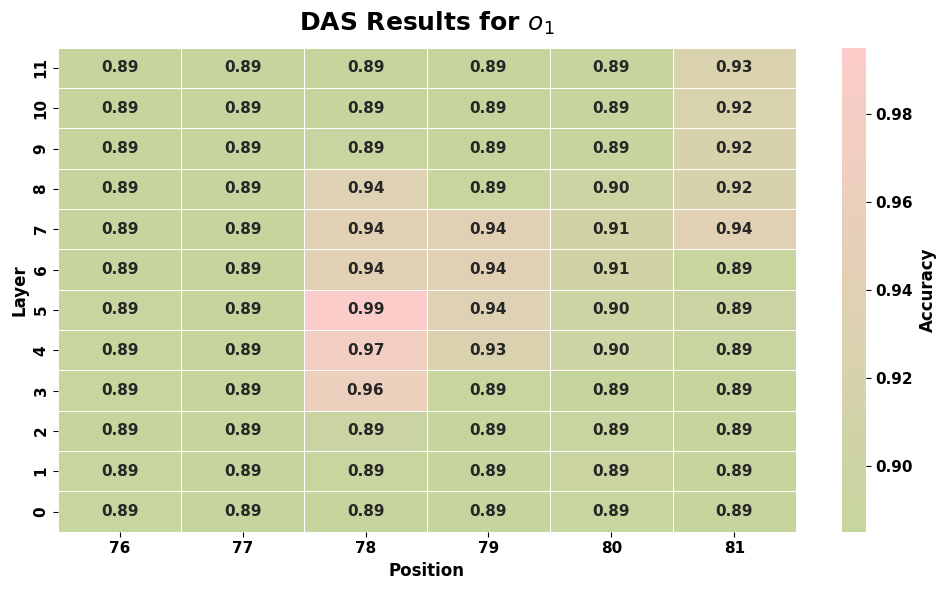
\includegraphics[width=\textwidth]{figs/das_heatmap_o1.png}
     \end{subfigure}
     \hfill
     \begin{subfigure}[b]{0.45\textwidth}
         \centering
         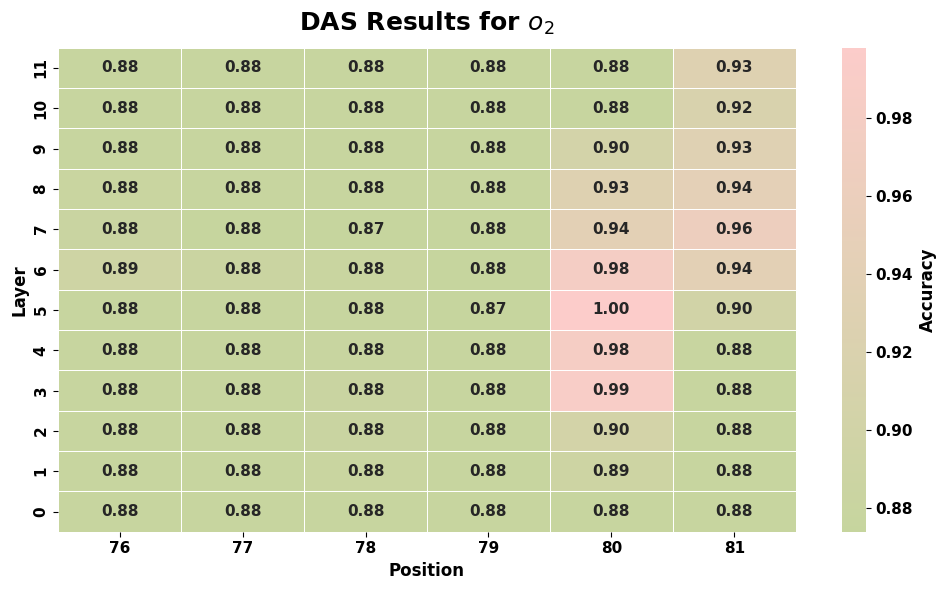
\includegraphics[width=\textwidth]{figs/das_heatmap_o2.png}
     \end{subfigure}

     \vspace{0.5cm} % Adds vertical spacing between rows

     % --- Second Row ---
     \begin{subfigure}[b]{0.45\textwidth}
         \centering
         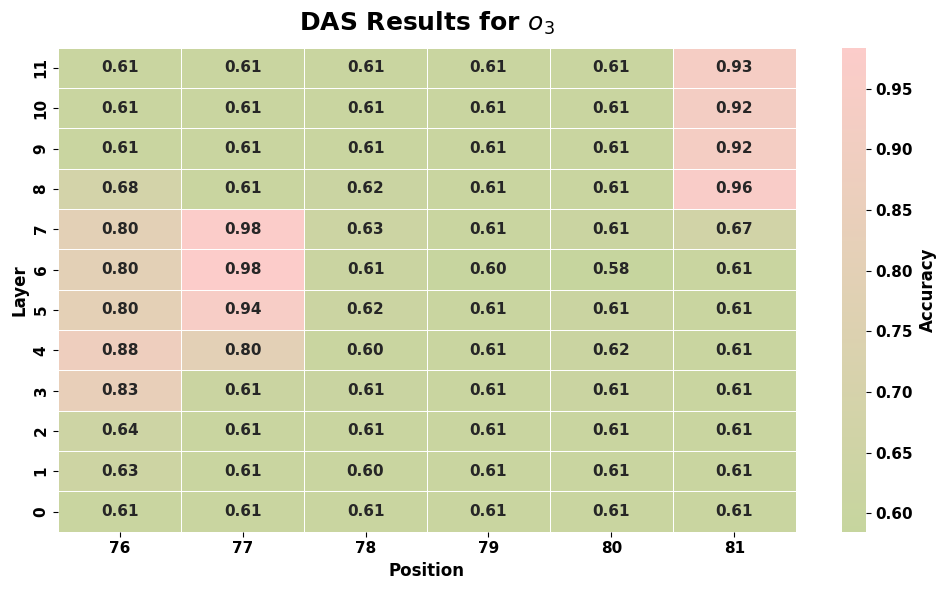
\includegraphics[width=\textwidth]{figs/das_heatmap_o3.png}
     \end{subfigure}
     \hfill
     \begin{subfigure}[b]{0.45\textwidth}
         \centering
         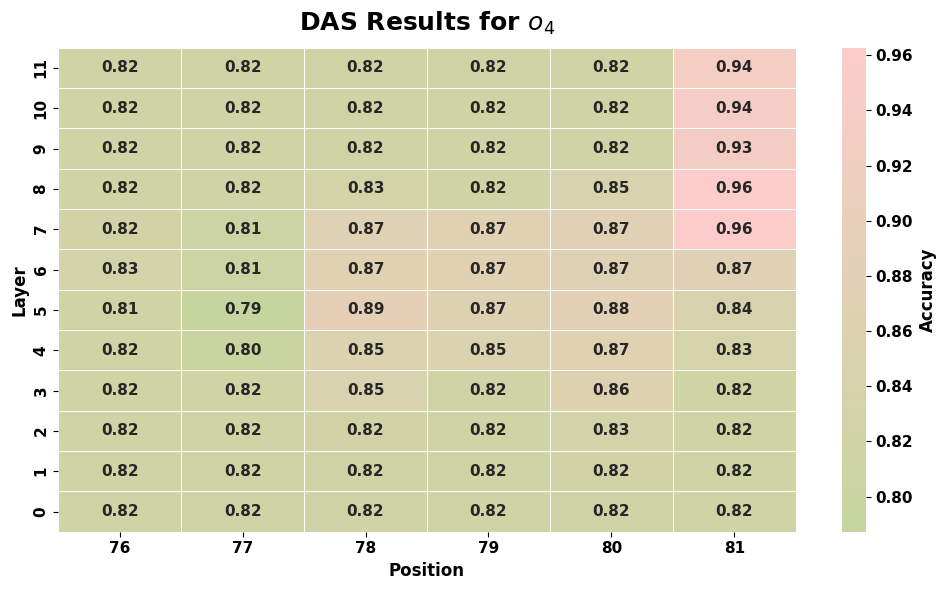
\includegraphics[width=\textwidth]{figs/das_heatmap_o4.png}
     \end{subfigure}
        
     \caption{DAS Alignment Heat Maps for $o_1,o_2,o_3,o_4$. }
     \label{fig:logic_das}
\end{figure}


\subsection{Diagnostic Graph Construction}
Once the optimal candidate layer and position for an intermediate variable are identified via DAS, we construct the Interchangeability Graph to diagnose the alignment's structural faithfulness. For $N$ sampled inputs from the filtered dataset, we perform exhaustive directed interventions for all pairs $(i, j)$ using the trained DAS weight. An undirected edge is drawn between node $i$ and node $j$ if and only if the interchange intervention succeeds bidirectionally---meaning the model accurately predicts the counterfactual output when patching from $i \rightarrow j$, and independently when patching from $j \rightarrow i$. 

\paragraph{Partitioning}
We partition the resulting graph using a heuristic multi-seed greedy quasi-clique search (\cref{alg:multi_seed_quasi}). To accommodate slight representational noise inherent to neural activations, we apply a density threshold of $\gamma = 0.98$ and a minimum clique size of 2. The resulting clusters explicitly separate the input space into perfectly-interpreted (interchange-consistent) regions and under-interpreted regions.

\subsection{SAE-Based Generalization and Classification}
To determine if the boundaries of the perfectly interpreted subspaces are explicitly encoded in the model's feature space, we train classifiers using SAE features to predict bucket membership.

\paragraph{Feature Extraction and Classification}
For the nodes in the intervention graph, we extract the residual-stream activations at the targeted layer and token position. We encode these activations using pretrained SAEs for GPT-2 Small (specifically, the \texttt{gpt2-small-res-jb} release from \texttt{sae\_lens}). Using the resulting sparse feature activations, we train an $\ell_1$-regularized Logistic Regression classifier on an 80/20 train/test split. The model is trained to classify whether an input belongs to the perfectly-interpreted bucket or the other bucket. The high test accuracy of this classifier and the sparse set of non-zero $\ell_1$ coefficients allow us to identify the specific features (such as $o_4$) that dictate whether the high-level causal hypothesis holds.




\section{Entity Binding Task Details}

\subsection{Task Specification and Dataset}
We instantiate the entity binding task using the \texttt{filling\_liquids} task family. In this setting, the model is provided with a prompt containing 10 distinct entity groups. Each group follows a fixed template: \textit{"[Person] fills a [Container] with [Liquid]."} The prompt concludes with a query such as \textit{"Who filled the [Container]?"}, requiring the model to retrieve the specific [Person] associated with that container from the preceding context.

\paragraph{Entity Pools} To ensure high diversity and minimize accidental overlaps, we utilize the following entity pools:
\begin{itemize}
    \item \textbf{Persons:} John, Mary, Bob, Sue, Tim, Kate, Dan, Lily, Max, Eva, Sam, Zoe, Leo, Mia, Noah, Ava, Ben, Liz, Tom, Joy.
    \item \textbf{Containers:} cup, glass, bottle, mug, jar, pitcher, bowl, flask, tumbler, chalice, vessel, container, tank, can, tube, vial, goblet, stein, carafe, decanter.
    \item \textbf{Liquids:} beer, wine, water, juice, milk, coffee, tea, soda, lemonade, smoothie, soup, broth, sauce, syrup, oil, honey, cider, nectar, punch, tonic.
\end{itemize}

\paragraph{Dataset Construction} We generate a dataset of 1,024 samples. Following our diagnostic pipeline, we filter this dataset to include only instances where \texttt{Gemma-2-2B-Instruct} correctly predicts the target entity for both the base and counterfactual inputs. After filtering, the dataset is split into training (80\%) and testing (20\%) sets.

\subsection{Experimental Setup}
We use \texttt{pyvene} to conduct vanilla interchange interventions. We test the \textit{positional hypothesis}, which posits that the model's retrieval mechanism is mediated by a high-level variable $q_{\mathrm{group}}$ representing the context position of the queried group. 

\paragraph{Alignment Procedure} Counterfactuals are generated by swapping the positions of entity groups while maintaining the templatic structure. We perform full-vector patching on the residual stream  at the final query token position across all layers. A faithful abstraction requires that patching the internal representation from a source input into a base input causes the model to retrieve the entity corresponding to the source's queried group position.

\subsection{Diagnostic Results}
We sample $512$ correctly answered prompts from the \texttt{filling\_liquids} input space, perform pairwise interchange interventions, and construct an Interchangeability Graph whose vertices represent individual inputs. We analyze the resulting IIA to construct the interchangeability graph shown in \cref{fig:InterchangeabilityGraph}. 

\begin{figure}[!htb]
    \centering
    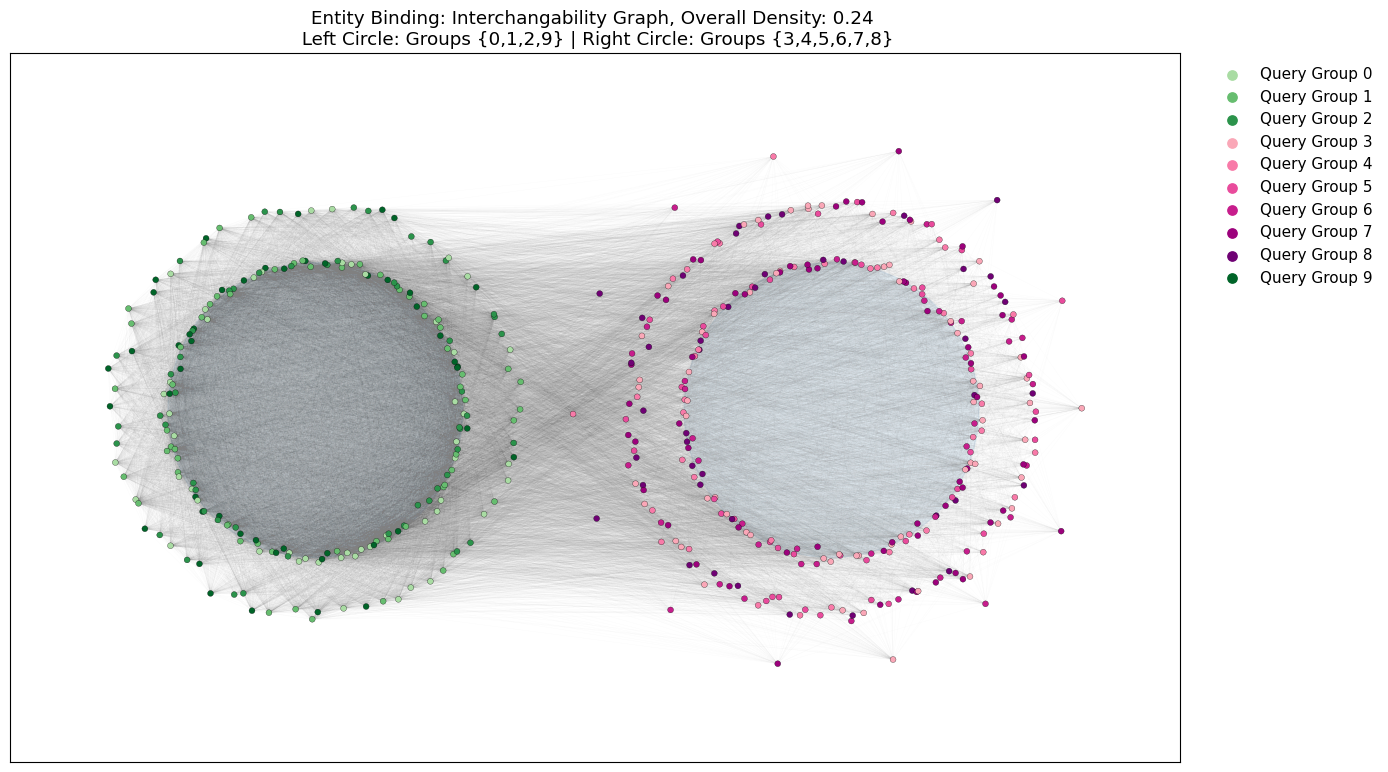
\includegraphics[width=0.7\linewidth]{figs/EntityBindingGraph.png}
    \caption{\textbf{Interchangeability Graph for Entity Binding.} The graph nodes represent individual inputs, and edges denote perfect pairwise interchangeability. The emergent community structure corresponds to the "Target Buckets" where the positional hypothesis is perfectly faithful, primarily at the start and end of the prompt sequence.}
    \label{fig:InterchangeabilityGraph}
\end{figure}

For the classification step of our diagnosis, we utilize internal features from \texttt{Gemma Scope} \cite{lieberum2024gemmascope} to determine if the boundaries between well-interpreted and under-interpreted regions are explicitly encoded in the model's feature space.

\section{Entangled Factual Recall Task Details}

\subsection{Task Specification and Dataset}
We evaluate the entangled factual recall setting using the RAVEL benchmark \citep{huang2024ravel} on the \texttt{Llama-3.1-8B} model. We focus on the \textsc{Language} attribute of the \textit{city} entity type. The input space consists of prompts where the base and source inputs share the exact same template but differ only in the city name (e.g., \textit{"People in San Francisco speak..."} vs. \textit{"People in Paris speak..."}). 

To ensure our interventions target the specific entity representation, we extract the residual stream activations at the final token of the city name. The dataset is filtered to strictly include instances where the base model correctly predicts the factual target. The filtered dataset is then split into an 80\% training set and a 20\% testing set.

\subsection{Experimental Setup: MDAS}
We employ Multi-task Distributed Alignment Search (MDAS) to learn a disentangled subspace that isolates the \textsc{Language} attribute from other co-encoded attributes (\textsc{Continent}, \textsc{Country}, \textsc{Latitude}, \textsc{Longitude}, and \textsc{Timezone}). 

\paragraph{MADS Loss}  Following \cite{huang2024ravel}, given an entity $E$ and an attribute $A$ with a ground-truth value $A_E$ (e.g., \textsc{Paris} and \textsc{Continent}), we seek to learn a feature $F_A$. A high \textbf{Cause} score indicates that intervening on this representation successfully transfers a source attribute value $A_{E'}$ from a counterfactual input $x'$ to the model's prediction for a base input $x$, optimized as:
\begin{equation}\label{eq:loss_cause}
\mathcal{L}_{Cause}(A, F_A, \mathcal{M}) = \text{CE}(\text{II}(\mathcal{M}, F_A, x, x'), A_{E'})
\end{equation}
Conversely, a high \textbf{Iso} (isolation) score ensures the intervention is surgical and does not alter other attributes $A^* \in \mathcal{A} \setminus \{A\}$. For a prompt $x^*$ querying a different attribute $A^*$ with ground-truth value $A_E^*$ (e.g., \textsc{Language}), the isolation loss ensures the model still predicts the original value $A_E^*$ despite the intervention on $F_A$:
\begin{equation}\label{eq:loss_iso}
\mathcal{L}_{Iso}(A, F_A, \mathcal{M}) = \frac{1}{|\mathcal{A} \setminus \{A\}|} \sum_{A^* \in \mathcal{A} \setminus \{A\}} \text{CE}(\text{II}(\mathcal{M}(x^*), F_A, x'), A_E^*)
\end{equation}
The MDAS training  loss is the summation of $\mathcal{L}_{Cause}$ and $\mathcal{L}_{Iso}$.  

\paragraph{Training Details} Rather than exhaustively training across all layers, we first perform a coarse search using a large layer gap across subspace dimensions $k \in \{32, 128, 512, 2048\}$. Based on the preliminary alignment results from this initial sweep, we zoom in on the most promising regions to localize the optimal subspace and identify layer 14 as the ideal intervention site. To optimize for both causal transfer and isolation, we construct a weighted training distribution: pairs evaluating the target attribute (\textsc{Language}) are sampled at a 5:1 ratio compared to pairs evaluating the other five off-target attributes. This forces the subspace to maximize the interchange intervention accuracy (IIA) for \textsc{Language} while ensuring interventions do not alter the model's predictions for queries about a city's continent or timezone.

\begin{figure}[!htb]
    \centering
    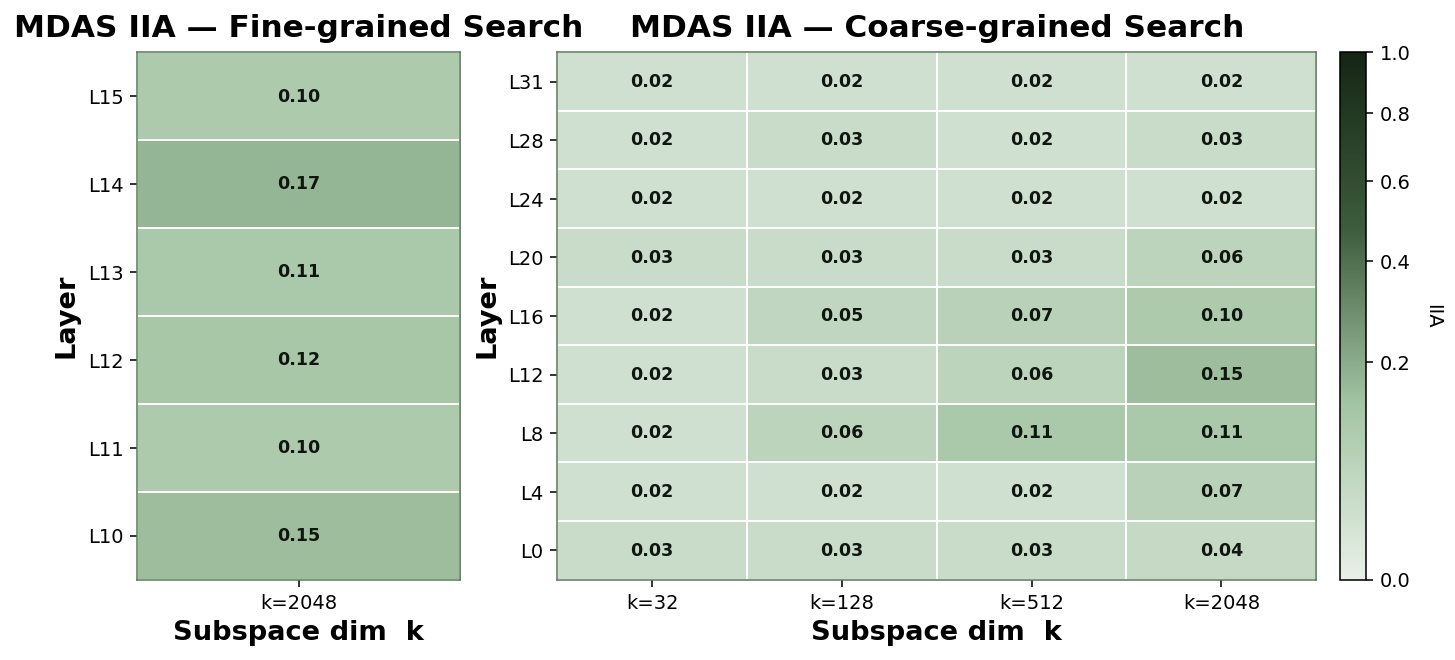
\includegraphics[width=0.5\linewidth]{figs/Engtanglemdas.png}
    \caption{MDAS Alignment Results for Entangled Factual Recall Task}
    \label{fig:mdas}
\end{figure}

\subsection{Diagnostic Results and Classification}
Following the MDAS optimization, we apply our diagnostic pipeline to the test set. 

\paragraph{Graph Construction and Partition} We perform exhaustive pairwise interchange interventions. An undirected edge is formed between two inputs if and only if the bidirectional interchange intervention (source $\rightarrow$ base, and base $\rightarrow$ source) is perfectly consistent with the high-level causal model. We partition this graph using \cref{alg:multi_seed_quasi} with a density threshold of $\gamma = 0.98$ and a minimum clique size of 2, which successfully isolates the language-specific clusters (English, Spanish) discussed in the main text. We find that with fewer buckets, the partition first separates English from non-English cities, and then Spanish splits off as a second clean group.

\paragraph{SAE-Based Generalization} To test if these boundaries are encoded in the model's internal feature space, we train a classifier using sparse features from \emph{Llama Scope} \citep{he2024llamascope}. We extract the residual stream activations at layer 14 for the graph nodes and encode them through the corresponding Llama SAE. 

Using the resulting sparse feature activations, we train a multi-class $\ell_1$-regularized Logistic Regression classifier to predict the quasi-clique bucket labels. To interpret the structural differences between buckets, we extract the highest-weight SAE features by analyzing the $\ell_1$ coefficients. 
 